%!TEX root = edance.tex
%%%%%%%%%%%%%%%%
%   CHAPTER 5  %
%%%%%%%%%%%%%%%%
\chapter{PN Junctions in Equilibrium}
\label{ch:ch05_pn_junc}
\graphicspath{{./figures/figs_ch05_pn_junc/}}
%%%%%%%%%%%%%%%%%%%%%%%%%%%%%%%%%%%%%%%%%%%%%%%%%%%%%%%%%%%%%%%%%%%%%%%%%%%%%%%%%%%%%%%%
%%%%%%%%%%%%%%%%%%%%%%%%%%%%%%%%%%%%%%%%%%%%%%%%%%%%%%%%%%%%%%%%%%%%%%%%%%%%%%%%%%%%%%%%
%                                   SECTION 5.1                                        %
%%%%%%%%%%%%%%%%%%%%%%%%%%%%%%%%%%%%%%%%%%%%%%%%%%%%%%%%%%%%%%%%%%%%%%%%%%%%%%%%%%%%%%%%
%%%%%%%%%%%%%%%%%%%%%%%%%%%%%%%%%%%%%%%%%%%%%%%%%%%%%%%%%%%%%%%%%%%%%%%%%%%%%%%%%%%%%%%%
\section{Chapter Preview}
We will see in this chapter and the following that the simple $PN$-junction structure provides a rich variety of functionality.  It can be used as a function of bias, acting as a "one way" gate for current, rectifying AC signals and allowing AC-to-DC conversion, converting light photons into electrical energy (solar cell), and performing the opposite functionality of creating light from electricity in a very efficient manner in light-emitting diodes (LEDs).  This simple structure is also the foundation of lasers and photo-detectors, used to transport energy around the globe using thin fibers of glass, imaging inside of the body, detecting x-rays and other high energy particles, among many other functions.  Diodes are also used to detect extremely high frequency signals, demodulating information in communication receivers, or used as switches to allow a transmitter and receiver to share the same antenna.  It is no exaggeration that the diode is one of the most versatile circuit elements.  To understand these myriad of applications, we must first discover the properties of the junction under a forward and reverse bias.  In this chapter we focus on the reverse bias, which is simpler to analyze.

We begin by considering that a concentration variation in carriers across a junction (such as a massive amount of electrons in an $N$-region compared to a dearth of electrons in a $P$-region) leads to a built-in potential difference between these regions.  We apply this to a $PN$-junction at thermal equilibrium to find its properties, including its ability to store charge as a non-linear capacitor.  In the next chapter, we will see how the diode conducts current.
%%%%%%%%%%%%%%%%%%%%%%%%%%%%%%%%%%%%%%%%%%%%
%                 FIGURE                   %
%%%%%%%%%%%%%%%%%%%%%%%%%%%%%%%%%%%%%%%%%%%%
% \begin{figure}[H]
% \centering
% \includegraphics[scale=1.00]{null}
% \caption{null}
% \label{fig:ch05_intro}
% \end{figure}
%%%%%%%%%%%%%%%%%%%%%%%%%%%%%%%%%%%%%%%%%%%%
\newpage
%%%%%%%%%%%%%%%%%%%%%%%%%%%%%%%%%%%%%%%%%%%%%%%%%%%%%%%%%%%%%%%%%%%%%%%%%%%%%%%%%%%%%%%%
%%%%%%%%%%%%%%%%%%%%%%%%%%%%%%%%%%%%%%%%%%%%%%%%%%%%%%%%%%%%%%%%%%%%%%%%%%%%%%%%%%%%%%%%
%                                   SECTION 5.2                                        %
%%%%%%%%%%%%%%%%%%%%%%%%%%%%%%%%%%%%%%%%%%%%%%%%%%%%%%%%%%%%%%%%%%%%%%%%%%%%%%%%%%%%%%%%
%%%%%%%%%%%%%%%%%%%%%%%%%%%%%%%%%%%%%%%%%%%%%%%%%%%%%%%%%%%%%%%%%%%%%%%%%%%%%%%%%%%%%%%%
\section{Structure}
As shown in \emph{Fig.~\ref{fig:slide2}}, a $PN$-junction is simply the junction between two regions doped as $N$-type and $P$-type.  When terminals are added to both sides, it is known as a $PN$-junction diode, or just a diode.
%%%%%%%%%%%%%%%%%%%%%%%%%%%%%%%%%%%%%%%%%%%%
%                 FIGURE                   %
%%%%%%%%%%%%%%%%%%%%%%%%%%%%%%%%%%%%%%%%%%%%
\begin{figure}[tb]
\centering
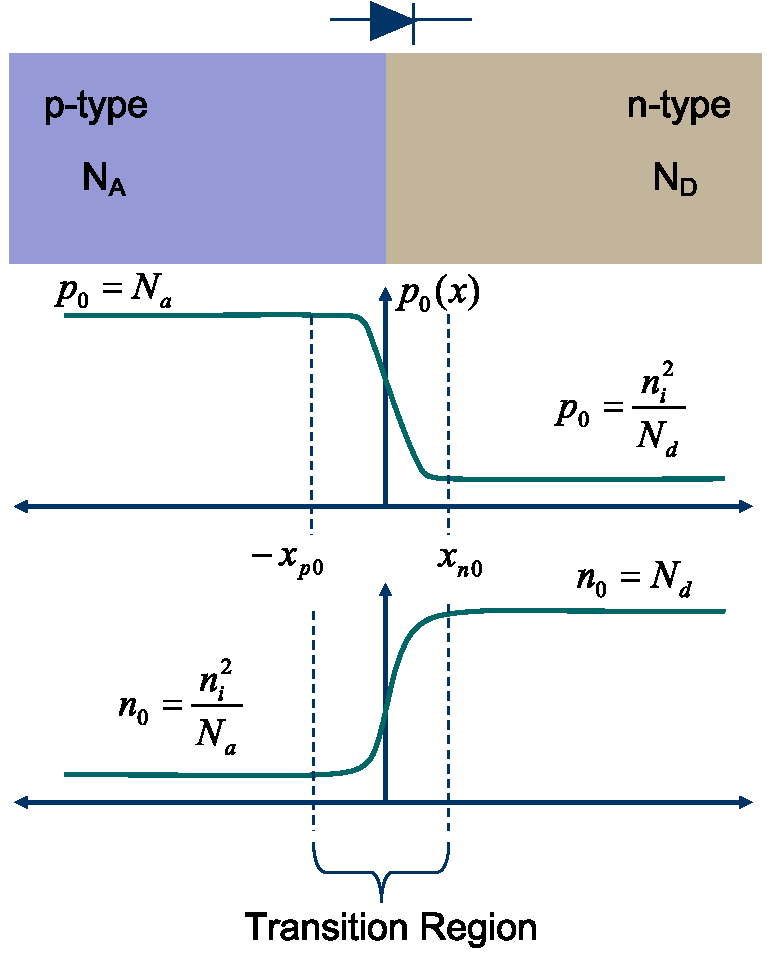
\includegraphics[width=.5\columnwidth]{slide2}
\caption{A $PN$-junction is the interface between a $P$-type and $N$-type doped semiconductor.  There are large concentration gradients between the two sides, with orders of magnitude more holes on the $P$-side compared to the $N$-side.  The same is true of electrons on the $N$-side.  Even though the junction is abrupt, we shall see that the concentration must change smoothly over a "transition region" from one region to the other.}
\label{fig:slide2}
\end{figure}
%%%%%%%%%%%%%%%%%%%%%%%%%%%%%%%%%%%%%%%%%%%%%%%%%%%%%%%%%%%%%%%%%%%%%%%%%%%%%%%%%%%%%%%%
%%%%%%%%%%%%%%%%%%%%%%%%%%%%%%%%%%%%%%%%%%%%%%%%%%%%%%%%%%%%%%%%%%%%%%%%%%%%%%%%%%%%%%%%
%                                   SECTION 5.3                                        %
%%%%%%%%%%%%%%%%%%%%%%%%%%%%%%%%%%%%%%%%%%%%%%%%%%%%%%%%%%%%%%%%%%%%%%%%%%%%%%%%%%%%%%%%
%%%%%%%%%%%%%%%%%%%%%%%%%%%%%%%%%%%%%%%%%%%%%%%%%%%%%%%%%%%%%%%%%%%%%%%%%%%%%%%%%%%%%%%%
\section{Carrier Concentration and Potential}
In \textbf{thermal equilibrium}\index{Thermal equilibrium}, under the assumption that there are no external fields, we expect the electron and hole current densities to be zero.  Recall that there might be a lot of motion due to thermal energy, but on average the currents should be zero.  If there is a steady-state concentration gradient that is somehow maintained, then that implies there is a constant diffusion current, which must be canceled by a corresponding drift current.  For the electrons we have:\footnote{Why not the sum of the electron and hole currents?}
    \begin{equation}
        J_n = 0 = q{n_0}{\mu _n}{\mathcal{E}_0} + q{D_n}\frac{{d{n_o}}}{{dx}} 
    \end{equation}
This equality between drift\index{Current!drift} and diffusion\index{Current!diffusion} implies that there must be a non-zero field $\mathcal{E}_0$.  Since the electric field is the gradient of potential, we also see that there is a corresponding change in potential due the concentration gradient:
    \begin{equation} 
        \frac{d{n_o}}{dx} = -\left( \frac{\mu_n}{D_n} \right){n_o}{\mathcal{E}_0} 
        = \left( \frac{q}{kT} \right){n_o}\frac{d{\varphi _0}}{dx} 
    \end{equation}
We have used Einstein's relation\index{Einstein's relation} $kT/q = D/\mu$ to simplify the equation.  The differential in voltage is related to the differential in concentration:
    \begin{equation} 
        d\varphi_0 = \left( \frac{kT}{q} \right)\frac{d{n_o}}{n_0} = V_{th}\frac{d{n_0}}{n_0} 
    \end{equation}
We have an equation relating the potential to the carrier concentration.  Integrating this relation:
    \begin{equation}
        \varphi_0(x) - \varphi_0(x_0) = V_{th}\ln \frac{n_0(x)}{n_0(x_0)}
    \end{equation}
This shows that the potential difference is related to the logarithm of the concentration difference, with $V_{th} = kT/q$ as the scaling constant (about $26\;mV$ at room temperature). 

It is customary (and confusing) to define the potential reference to be intrinsic $Si$, or in other words, if an $N$-type region forms a junction with intrinsic silicon, it will develop a potential $\varphi$ derived from this equation:
    \begin{equation} 
        n = n_ie^{\varphi_0(x)/V_{th}}
    \end{equation}
    \begin{equation} 
        \varphi_n = V_{th} \ln\left( \frac{n}{n_i} \right)
    \end{equation}
If we do a similar calculation for holes, we need to carefully account for the fact that there are fewer electrons($n_p$) than intrinsic silicon($n_i$), making the potential negative:
    \begin{equation} 
        \varphi_p = V_{th} \ln\left( \frac{n_p}{n_i}  \right)
    \end{equation}
    \begin{equation} 
        \varphi_p = V_{th} \ln\left( \frac{n_i^2}{p \cdot n_i}  \right)
    \end{equation}
or:
    \begin{equation} 
        \varphi_p = V_{th} \ln\left( \frac{n_i}{p}  \right) = - V_{th} \ln\left( \frac{p}{n_i}  \right) 
    \end{equation}
Since this is an equilibrium situation, the Law of Mass Action\index{Law of mass action} should hold.  With these definitions of potential, we can express the free carrier density as $n_i$ times an exponential factor that takes the potential of the $P$-type or $N$-type region into account.  As expected, the Law of Mass Action is upheld:
    \begin{equation} 
        {n_0}(x){p_0}(x) = n_i^2{e^{ - {\varphi _0}(x)/{V_{th}}}}{e^{{\varphi _0}(x)/{V_{th}}}} = n_i^2 
    \end{equation}
%%%%%%%%%%%%%%%%%%%%%%%%%%%%%%%%%%%%%%%%%%%%
%              SUB-SUBSECTION              %
%%%%%%%%%%%%%%%%%%%%%%%%%%%%%%%%%%%%%%%%%%%%
\subsubsection{The Doping Changes Potential}
Due to the logarithmic nature of the potential, the potential changes linearly for exponential increase in doping:
    \begin{equation} 
        \varphi _0(x) = V_{th} \ln \frac{n_0(x)}{n_i(x_0)} = 26\;mV \cdot \ln \frac{n_0(x)}{n_i(x_0)} 
        \approx 26\;mV \cdot \ln 10\,\log \frac{n_0(x)}{{10}^{10}} 
    \end{equation}
\newpage
Since working with factors of ten is convenient when dealing with doping levels, we can convert these equations into a base 10 logarithm:
    \begin{equation} 
        {\varphi _0}(x) \approx 60{\rm{mV}}\,\,\log \frac{{{n_0}(x)}}{{{{10}^{10}}}} 
    \end{equation}
    \begin{equation} 
        {\varphi _0}(x) \approx  - 60{\rm{mV}}\,\,\log \frac{{{p_0}(x)}}{{{{10}^{10}}}} 
    \end{equation}
For example, to quickly calculate the potential of a $P$-type region with a concentration of $10^{16} \mathrm{cm}^{-3}$ holes, use the fact that we have 6 orders of magnitude more holes than intrinsic, so the potential is $6 \times 60\mathrm{mV} = -360 $mV.  A negative voltage means we are dealing with a $P$-type material.  An $N$-type materials has a positive potential with respect to intrinsic Si.
%%%%%%%%%%%%%%%%%%%%%%%%%%%%%%%%%%%%%%%%%%%%%%%%%%%%%%%%%%%%%%%%%%%%%%%%%%%%%%%%%%%%%%%%
%%%%%%%%%%%%%%%%%%%%%%%%%%%%%%%%%%%%%%%%%%%%%%%%%%%%%%%%%%%%%%%%%%%%%%%%%%%%%%%%%%%%%%%%
%                                   SECTION 5.4                                        %
%%%%%%%%%%%%%%%%%%%%%%%%%%%%%%%%%%%%%%%%%%%%%%%%%%%%%%%%%%%%%%%%%%%%%%%%%%%%%%%%%%%%%%%%
%%%%%%%%%%%%%%%%%%%%%%%%%%%%%%%%%%%%%%%%%%%%%%%%%%%%%%%%%%%%%%%%%%%%%%%%%%%%%%%%%%%%%%%%
\section{\emph{PN}-Junction in Equilibrium}
%%%%%%%%%%%%%%%%%%%%%%%%%%%%%%%%%%%%%%%%%%%%
%             SUBSECTION 5.4.1             %
%%%%%%%%%%%%%%%%%%%%%%%%%%%%%%%%%%%%%%%%%%%%
\subsection{\emph{PN}-Junction: Overview}
As illustrated in \emph{Fig.~\ref{fig:slide9}}, it is useful to do a thought experiment and consider what happens before we reach \textbf{equilibrium}\index{PN-junction!equilibrium}. Consider when the junction shown in \emph{Fig.~\ref{fig:slide2}} is first formed.  Due to the abrupt nature of the junction, we expect very large diffusion currents to flow.  Mobile charges transfer near the junction, especially majority carriers diffuse in large numbers.  The currents are large due to the large concentration gradients.  There are orders of magnitude more electrons in the $N$-type region, and orders of magnitude more holes in the $P$-type region.  So it is natural to assume that these carriers will diffuse to the other side, becoming minority carriers.  However, since these mobile carriers become minority carriers in the new region, they will not penetrate far due to recombination.

The key observation is that initially the two regions are charge neutral.  But as holes and electrons are charge carriers, as they cross the junction, they disturb the delicate charge balance and introduce net charge into each region.  As a result, a voltage difference builds up between regions.  This voltage gets larger and larger as more mobile carriers diffuse across the barrier.   This creates a field at the junction that causes drift currents to oppose the diffusion current.  This will ensue until the field is sufficiently large to produce a drift current that can counter the diffusion current.  In thermal equilibrium, drift current and diffusion must balance each other on average.  We will also show that near the junction a "transition region" develops so that the density of holes $p(x)$ and electrons $n(x)$ change smoothly from one side to the other.
\newpage
%%%%%%%%%%%%%%%%%%%%%%%%%%%%%%%%%%%%%%%%%%%%
%                 FIGURE                   %
%%%%%%%%%%%%%%%%%%%%%%%%%%%%%%%%%%%%%%%%%%%%
\begin{figure}[H]
\centering
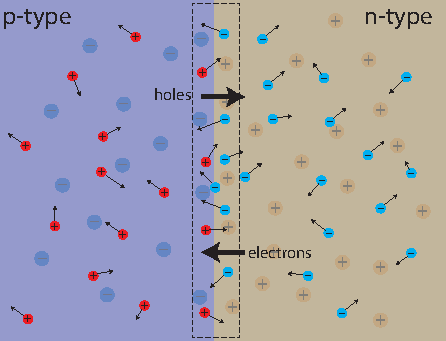
\includegraphics[width=.6\columnwidth]{pn_flow1}\\
(a)\\[0.25cm]
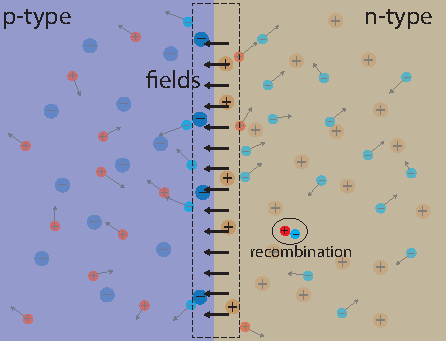
\includegraphics[width=.6\columnwidth]{pn_flow2}\\
((b)\\[0.25cm]
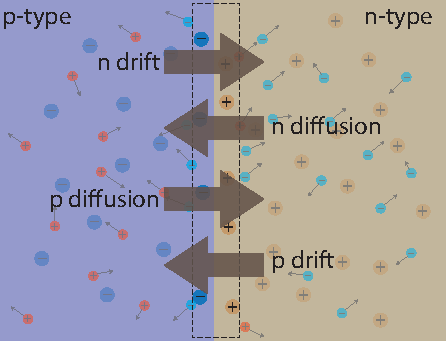
\includegraphics[width=.6\columnwidth]{pn_flow3}\\
(c)\\[0.25cm]
\caption{Here we outline the non-equilibrium situation when a contact between the $N$-type and $P$-type regions are formed.  (a)  Diffusion currents flow due to the large concentration gradients.  (b)  Charge imbalance leads to a potential barrier between the two regions.  (c) This internal \emph{built-in} potential leads to an equilibrium state with zero net current, whereby diffusion currents are balanced by drift currents.}
\label{fig:slide9}
\end{figure}
%%%%%%%%%%%%%%%%%%%%%%%%%%%%%%%%%%%%%%%%%%%%
\newpage
%%%%%%%%%%%%%%%%%%%%%%%%%%%%%%%%%%%%%%%%%%%%
%             SUBSECTION 5.4.2             %
%%%%%%%%%%%%%%%%%%%%%%%%%%%%%%%%%%%%%%%%%%%%
\subsection{\emph{PN}-Junction Currents}
Considering the $PN$-junction in thermal equilibrium,  the currents have to be zero.  So, we have for the electrons the same set of equations we derived earlier:
    \begin{equation} 
        J_n = 0 = q{n_0}{\mu _n}{\mathcal{E}_0} + q{D_n}\frac{dn_o}{dx}
    \end{equation}
    \begin{equation} 
        q{n_0}{\mu _n}{\mathcal{E}_0} =  - q{D_n}\frac{dn_o}{dx}
    \end{equation}
Now let's focus on the electric field, rather than the potential:
    \begin{equation} 
        \mathcal{E}_0 = \frac{-D_n\frac{dn_o}{dx}} {n_0\,\mu_n} = -\frac{kT}{q}\frac{1}{n_0}\frac{dn_0}{dx} 
    \end{equation}
We can also state the same applies for the holes:
    \begin{equation} 
        \mathcal{E}_0 = \frac{D_p\frac{dp_o}{dx}} {p_0\,\mu_p} = \frac{kT}{q}\frac{1}{p_0}\frac{dp_0}{dx} 
    \end{equation}
Since the fields must be finite, the concentration of electrons and holes cannot change abruptly. Therefore, a smooth variation is expected in the "transition region".  This is shown schematically in \emph{Fig.~\ref{fig:slide11}}.
%%%%%%%%%%%%%%%%%%%%%%%%%%%%%%%%%%%%%%%%%%%%
%                 FIGURE                   %
%%%%%%%%%%%%%%%%%%%%%%%%%%%%%%%%%%%%%%%%%%%%
\begin{figure}[H]
\centering
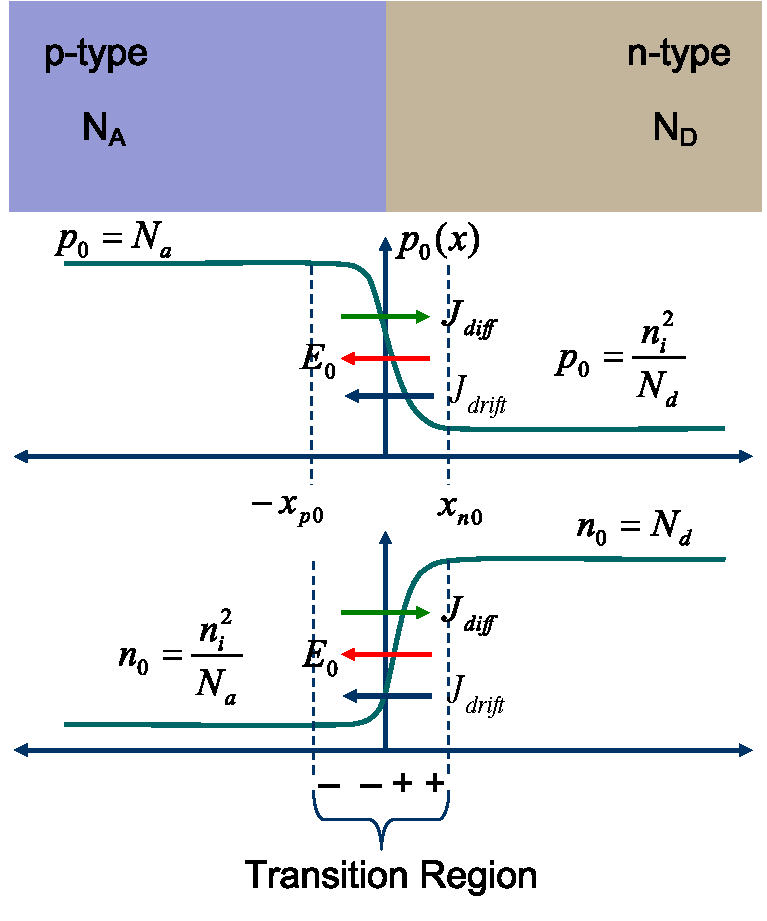
\includegraphics[width=.65\columnwidth]{slide11}
\caption{The concentration of electrons and holes changes smoothly from one region to the other.  The net charge at the boundary "space charge" region leads to an internal electric field which produces a drift current that balances the equilibrium diffusion current.}
\label{fig:slide11}
\end{figure}
%%%%%%%%%%%%%%%%%%%%%%%%%%%%%%%%%%%%%%%%%%%%
\newpage
%%%%%%%%%%%%%%%%%%%%%%%%%%%%%%%%%%%%%%%%%%%%
%             SUBSECTION 5.4.3             %
%%%%%%%%%%%%%%%%%%%%%%%%%%%%%%%%%%%%%%%%%%%%
\subsection{\emph{PN}-Junction Fields}
With reference to \emph{Fig.~\ref{fig:slide11}}, let's define the transition region width as $x_{p_0}$ and $x_{n_0}$, where the first subscript denotes the region type, and the second subscript emphasizes thermal equilibrium\index{Thermal equilibrium}.  The \textbf{transition regions}\index{PN-junction!transition region} are defined as the region near the junction where the majority carrier concentrations deviate from the equilibrium values for an isolated doped semiconductor.  To solve for the electric fields, we need to write down the charge density in each region:
    \begin{equation} 
        \rho _0(x) = q(p_0 - n_0 + N_D - N_A) 
    \end{equation}
On the $P$-side of the junction, there are very few electrons and only acceptors:
    \begin{align} 
        \rho _0(x) &\approx q(p_0 - N_A) &\textit{for $-x_{p_0} < x < 0$} 
    \end{align}
Since the hole concentration is decreasing on the $P$-side, the net charge is negative:
    \begin{equation} 
        {N_A} > {p_0} 
    \end{equation}
and so
    \begin{equation}
        {\rho _0}(x) < 0 
    \end{equation}
Analogous to the $P$-side, the charge on the $N$-side is given by:
    \begin{align} 
        \rho _0(x) &\approx q(-n_0 + N_D) &\textit{for $0 < x < x_{n_0}$} 
    \end{align}
The net charge here is positive since:
    \begin{equation} 
        N_D > n_0 
    \end{equation}
So we have:
    \begin{equation} 
        \rho _0(x) > 0 
    \end{equation}
These facts are summarized in \emph{Fig.~\ref{fig:slide11}}.  We see a field arising that begins with the positive charges ($N$-side), and ends on the negative charges ($P$-side) inside the transition region\index{PN-junction!transition region}.  By definition, the transition region is therefore the region where the charge density is non-zero.  Note that normal $N$-type and $P$-type materials are charge neutral, because ionized dopant charges are neutralized by an equal number of free carriers.  In the transition region, the free carriers are depleted (due to diffusion) and so there is net charge.   
%\begin{figure}[tb]
%\centering
%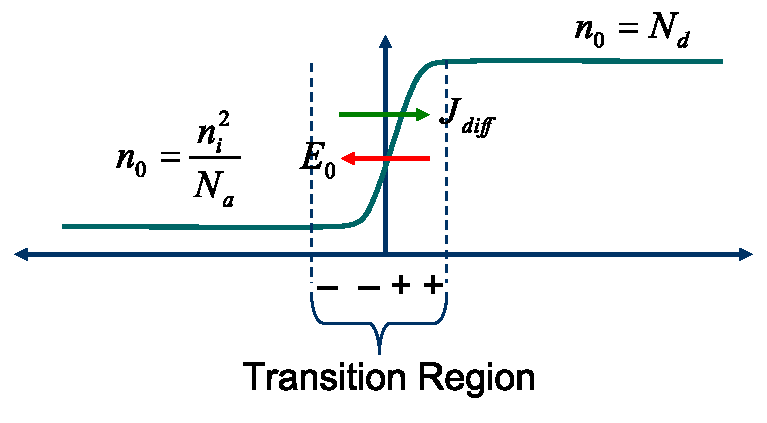
\includegraphics[width=.5\columnwidth]{slide13}
%\caption{slide 13 } \label{fig:slide13}
%\end{figure}
%%%%%%%%%%%%%%%%%%%%%%%%%%%%%%%%%%%%%%%%%%%%
%             SUBSECTION 5.4.4             %
%%%%%%%%%%%%%%%%%%%%%%%%%%%%%%%%%%%%%%%%%%%%
\subsection{“Exact” Equation for Fields}
Given the above approximations, we now have an expression for the \textbf{charge density}\index{PN-junction!charge density} in each region of the semi-conductor:
    \begin{equation}
        \rho _0(x) \cong
            \begin{cases} 
                q(n_i{e^{-\varphi_0(x)/V_{th}}} - {N_A}) &,\; -x_{p_o} < x < 0 \\ \\
                q(N_D - n_i\,{e^{\varphi_0(x)/V_{th}}}) &,\; 0 < x < x_{n_0}
            \end{cases}
    \end{equation}
We also have the following result from electrostatics:
    \begin{equation} 
        \frac{d{\mathcal{E}_0}}{dx} = -\frac{d^2\varphi}{dx^2} = \frac{\rho_0(x)}{\varepsilon_s}
    \end{equation}
Notice that the potential $\varphi$ appears on both sides of the equation, making it difficult to solve the problem.   We can find a much simpler equation to solve if we make a simplifying assumption about the charge in the transition region, known as the depletion approximation.
%%%%%%%%%%%%%%%%%%%%%%%%%%%%%%%%%%%%%%%%%%%%
%             SUBSECTION 5.4.5             %
%%%%%%%%%%%%%%%%%%%%%%%%%%%%%%%%%%%%%%%%%%%%
\subsection{Depletion Approximation}
The \textbf{depletion approximation}\index{PN-junction!depletion approximation} is simply that all free carriers are "depleted" in the transition region, making the entire region consist of ionized dopants.  Under this assumption, the charge density expressions are independent of the potential, and are constant:
    \begin{equation}
        \rho _0(x) \cong
            \begin{cases} 
                -q\,N_A &,\; -x_{p_o} < x < 0 \\ \\
                (+)q\,N_D &,\; 0 < x < x_{n_0}
            \end{cases}
    \end{equation}
This implies the rate of change of the electric field is constant:
    \begin{equation} 
        \frac{{d{\mathcal{E}_0}}}{{dx}} = \frac{{{\rho _0}(x)}}{{{\varepsilon _s}}}
    \end{equation}
The solution for electric field is now easy and simply given by the integration of the charge over the region of interest:
    \begin{equation}
        \mathcal{E}_0(x) = \int_{-x_{p_0}}^x \frac{\rho _0(x')}{\varepsilon_s}dx' + \mathcal{E}_0(-x_{p_0}) 
    \end{equation}
Is the depletion approximation reasonable?  Note that in equilibrium, doped silicon is charge neutral because for every ionized dopant, there is a free carrier (of opposite sign).  As we derived earlier, the number of free carriers diminishes \textit{exponentially} as we go into the depletion region.  The potential voltage changes across the junction, a result we derived from stating that in equilibrium the net  current is zero.  The potential change is in fact the potential barrier that must arise as to counter the diffusion of carriers across the $PN$-junction.   From the $N$-side (higher potential) we move to the $P$-side, and the potential drops by $\sim.7\,V$ (depending on the doping).  For every $60\,mV$ drop in potential, there is a $10\,\times$ reduction in free carriers.  Since the free carrier concentration starts at the doping level and drops by $10\,\times$ for the first $60\,mV$ drop, we see that neglecting the free carrier concentration is actually quite a reasonable assumption to make and should only result in a very small error in the following calculations.

Returning to the solution of the problem, since charge density is a constant:
    \begin{equation} 
        \mathcal{E}_0(x) = \int_{-x_{p_0}}^x {\frac{\rho_0(x')}{\varepsilon_s}dx'} = -\frac{q{N_A}}{\varepsilon_s}(x + x_{po}) 
    \end{equation}
If we start from the $N$-side we get the following result:
    \begin{equation} 
        \cancel{\mathcal{E}_0(x_{n_0})} = \int_x^{x_{n_0}} {\frac{{\rho_0}(x')}{\varepsilon_s}dx'} + \mathcal{E}_0(x) =  \frac{q\,N_D}{\varepsilon_s}(x_{n_0} - x) + \mathcal{E}_0(x) 
    \end{equation}
or:
    \begin{equation} 
        \mathcal{E}_0(x) = -\frac{q\,N_D}{\varepsilon_s}(x_{n_0} - x)
    \end{equation}
Since we impose that $\mathcal{E}_0(x_{n_0}) = 0$ outside of the transition region.  This is also reasonable because in the neutral $PN$-junction regions, the fields are zero under equilibrium (no external fields are applied either).  
%%%%%%%%%%%%%%%%%%%%%%%%%%%%%%%%%%%%%%%%%%%%
%              SUB-SUBSECTION              %
%%%%%%%%%%%%%%%%%%%%%%%%%%%%%%%%%%%%%%%%%%%%
\subsubsection{Plot of Fields In Depletion Region}
%%%%%%%%%%%%%%%%%%%%%%%%%%%%%%%%%%%%%%%%%%%%
%                 FIGURE                   %
%%%%%%%%%%%%%%%%%%%%%%%%%%%%%%%%%%%%%%%%%%%%
\begin{figure}[H]
\centering
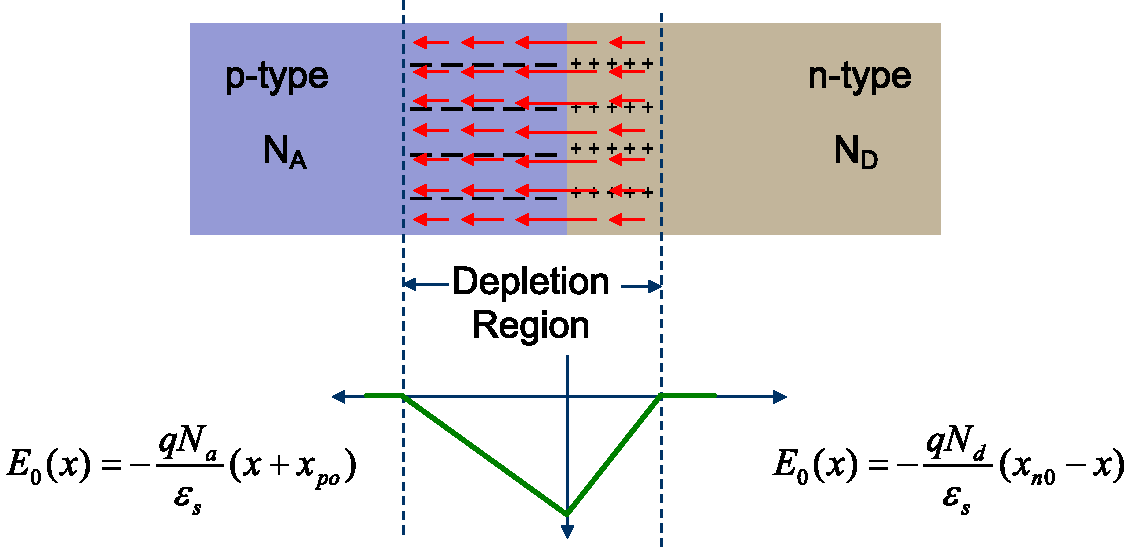
\includegraphics[width=\columnwidth]{slide18}
\caption{The electric fields in the depletion region are negative (they point left since the positive charges are on the right and the negative charges are on the left).  Here we assume zero fields in the neutral $P$-region and $N$-region.  The peak fields occur at the junction.}
\label{fig:slide18}
\end{figure}
%%%%%%%%%%%%%%%%%%%%%%%%%%%%%%%%%%%%%%%%%%%%
In \emph{Fig.~\ref{fig:slide18}} we plot the electric fields across the $PN$-junction.  Note that the electric field is zero outside of the depletion region, and the electric field grows uniformly as we enter the depletion region.  If we start on the $P$-side, the fields gradually grow from zero to a peak value at the interface of the region.  Then as we enter the $N$-side, the electric field grows back down to zero as we enter the neutral $N$-region.  

There are several noteworthy facts to take away from this plot.  First the width of the depletion region is not necessarily symmetric between the $N$-side and $P$-side.  Also, the slope of the electric field is larger in one region than the other.  Finally the negative peak of the field always occurs at the junction.  Why is that?

All of these facts are explained by the difference in doping levels between the $N$-type and $P$-type side.  The region with the higher doping will have a smaller depletion region because it can support more charge per unit volume.  Also, the peak is always at the junction or transition point because fields originate because of charge.  From Gauss' law\index{Gauss' law} we know that if we were to draw an imaginary box around the $P$-region, with one face of the box intersecting the neutral $P$-region, and the other face crossing the depletion region, then as we move the second face to the right into the $P$-region, we are covering more and more charge inside the box, causing the fields crossing the boundary to be necessarily larger.  This is true until the boundary crosses the origin and enters the $N$-region.  Now the amount of charge begins to decrease because we have both positive and negative charges in the box.  Finally, when the box reaches the neutral $N$-region, it must contain exactly zero charge, or stated another way, the amount of charge uncovered in the depletion regions must be equal and opposite in magnitude.
%%%%%%%%%%%%%%%%%%%%%%%%%%%%%%%%%%%%%%%%%%%%
%              SUB-SUBSECTION              %
%%%%%%%%%%%%%%%%%%%%%%%%%%%%%%%%%%%%%%%%%%%%
\subsubsection{Continuity of the Electric Field Across the Junction}
The electric fields diverges on charge. For a sheet charge at the interface, the electric field could be discontinuous.   In our case, the depletion region is only populated by a background density of fixed charges so the electric field is continuous.  In other words, across the interface we have:
    \begin{equation} 
        {{\mathcal{E}_0}^n}\big\rvert_{x = 0} = -\frac{q\,N_A}{\varepsilon_s}{x_p}_o =  
        -\frac{q\,N_D}{\varepsilon_s}{x_n}_o = {{\mathcal{E}_0}^p}\big\rvert_{x = 0} 
    \end{equation}
Which is just another way of saying:
    \begin{equation} 
        q\,N_A\,x_{p_0} = q\,N_D\,x_{n_0} 
    \end{equation}
Or in words, the total fixed charge in the $N$-region equals the total fixed charge in the $P$-region.  This is of course something we already anticipated from Gauss' Law.
%%%%%%%%%%%%%%%%%%%%%%%%%%%%%%%%%%%%%%%%%%%%
%              SUB-SUBSECTION              %
%%%%%%%%%%%%%%%%%%%%%%%%%%%%%%%%%%%%%%%%%%%%
\subsubsection{Potential Across Junction}
From our earlier calculation we know that the potential in the $N$-region is higher than the  $P$-region.  We also noted that the potential has to smoothly transition from high to low in crossing the junction.   We know that the physical origin of the potential difference is due to the charge transfer that occurred due to the concentration gradient.   Let's integrate the field to get an analytical expression for the potential:
    \begin{equation*}
        \varphi(x) = \varphi(-x_{p_0}) + \int_{-x_{p_0}}^{x} \frac{q\,N_A}{\varepsilon_s}(x' + x_{p_0})dx' 
    \end{equation*}
This integral is easy to perform:
    \begin{equation*}
        \varphi(x) = \varphi_p + \frac{q\,N_A}{\varepsilon_s}
                    \left( {\frac{{x{'^2}}}{2} + x'x_{p_0}} \right)
                    \big\vert_{-x_{p_0}}^x 
    \end{equation*}
We arrive at potential on $P$-side:
    \begin{equation*}
        \varphi_0^p(x) = \varphi_p + \frac{q\,N_A}{2\,\varepsilon_s}{(x + {x_{p_0})}^2} 
    \end{equation*}
Also performing the integral on $N$-side:
    \begin{equation*}
        \varphi_0^n(x) = \varphi_n - \frac{q\,N_D}{2\,\varepsilon_s}{(x - {x_{n_0})}^2} 
    \end{equation*}
The potential \textit{must} be continuous at interface (field finite at interface)
    \begin{equation*}
        \varphi_0^n(0) = \varphi_n - \frac{q\,N_D}{2\,\varepsilon_s}{{x_{n_0}}^2} 
                        = \varphi_p + \frac{q\,N_A}{2\,\varepsilon_s}{{x_{p_0}}^2} = \varphi_0^p(0)
    \end{equation*}
%%%%%%%%%%%%%%%%%%%%%%%%%%%%%%%%%%%%%%%%%%%%
%              SUB-SUBSECTION              %
%%%%%%%%%%%%%%%%%%%%%%%%%%%%%%%%%%%%%%%%%%%%
\subsubsection{Solve for Depletion Lengths}
We have two equations and two unknowns. We are finally in a position to solve for the depletion depths:
    \begin{equation*} 
        \varphi_n - \frac{q\,N_D}{2\,\varepsilon_s}{x_{n_0}}^2 = \varphi_p + \frac{q\,N_A}{2\,\varepsilon_s}{x_{p_0}}^2 
    \end{equation*}
    \begin{equation*} 
        q\,N_A\,x_{p_0} = q\,N_D\,x_{n_0} 
    \end{equation*}
The solutions to these equations is given by:
    \begin{align} 
        \Aboxed{ x_{n_0} &= \sqrt{ \frac{2\,\varepsilon_s\varphi_{bi}}{q\,N_D} \left( \frac{N_A}{N_A + N_D} \right) } }
        &\textit{Depletion width on N-side}
    \end{align}
and:
    \begin{align}
        \Aboxed{ x_{p_0} &= \sqrt{ \frac{2\,\varepsilon_s\varphi_{bi}}{q\,N_A} \left( \frac{N_D}{N_A + N_D} \right) } }
        &\textit{Depletion width on P-side}
    \end{align}
Where the total potential difference between the $N$-type and $P$-type side is \textbf{built-in potential}\index{PN-junction!built-in potential}:
    \begin{equation}
        \varphi_{bi} \equiv \varphi_n - \varphi_p > 0 
    \end{equation}
%%%%%%%%%%%%%%%%%%%%%%%%%%%%%%%%%%%%%%%%%%%%
%              SUB-SUBSECTION              %
%%%%%%%%%%%%%%%%%%%%%%%%%%%%%%%%%%%%%%%%%%%%
\subsubsection{Sanity Check}
Does the above equation make sense?  Let's say we dope one side very highly. Then physically we expect the depletion region width for the heavily doped side to approach zero:
    \begin{equation} 
        x_{n_0} = \mathop{\lim}\limits_{{N_D} \to \infty}
                    \sqrt{\frac{2\,\varepsilon_s\,\varphi_{bi}}{q\,N_D} \frac{N_A}{N_D + N_A}} = 0 
    \end{equation}
Also for the depletion region on the $P$-side, the width should be independent of the doping level $N_D$:
    \begin{equation} 
        x_{p_0} = \mathop{\lim}\limits_{{N_A} \to \infty}
                    \sqrt{\frac{2\,\varepsilon_s\,\varphi_{bi}}{q\,N_A} \frac{N_D}{N_D + N_A}} = 
                    \sqrt{\frac{2\,\varepsilon_s\,\varphi_{bi}}{q\,N_A}}
    \end{equation}
We see that the entire depletion width is dropped across $P$-region, as expected.
%%%%%%%%%%%%%%%%%%%%%%%%%%%%%%%%%%%%%%%%%%%%
%             SUBSECTION 5.4.6             %
%%%%%%%%%%%%%%%%%%%%%%%%%%%%%%%%%%%%%%%%%%%%
\subsection{Total Depletion Width}
The sum of the depletion widths is the \textbf{“space-charge region”}\index{Space-charge region}:
    \begin{align}
        \Aboxed{ X_{{dep}_0} &= x_{p_0} + x_{n_0} = 
        \sqrt{ \frac{2\,\varepsilon_s\,\varphi_{bi}}{q} \left( \frac{1}{N_A} + \frac{1}{N_D} \right) } }
        &\textit{Total depletion region width}
    \end{align}
By definition, this region is essentially depleted of all mobile charge.  Due to high electric field, carriers move across region at velocity saturated speeds.  For example:
    \begin{equation} 
        X_{{dep}_0} = \sqrt{ \frac{2\,\varepsilon_s\,\varphi_{bi}}{q} \left( \frac{1}{{10}^{15}} \right) } \approx 1\,\mu
    \end{equation}
implies:
    \begin{equation} 
        \mathcal{E}_{pn-junction} \approx \frac{1\,V}{1\,\mu} = {10}^4\frac{V}{cm} 
    \end{equation}
The expression for the built-in potential is given by:
    \begin{equation*} 
        \varphi_{bi} \equiv \varphi_n - \varphi_p
        = V_T\,\Bigg( \ln \bigg( \frac{N_D}{n_i} \bigg) + \ln \bigg( \frac{N_A}{n_i} \bigg) \Bigg)
    \end{equation*}
    \begin{align}
        \Aboxed{ \varphi_{bi} &= V_T\,\ln \left( \frac{N_D\,N_A}{{n_i}^2} \right) }
        &\textit{Built-in potential}
        \label{eq:bi_voltage}
    \end{align}
In \emph{Eq.~\ref{eq:bi_voltage}}, $V_T$ (also often symbolized as $\phi_T$) is known as \textbf{thermal voltage}\index{Thermal voltage}, and it is equivalent to $k\,T/q \approx 26\,mV$.
Plugging in some typical numerical values for doping, we arrive at:
    \begin{equation} 
        \varphi_{bi} = 26\,mV \ln \frac{N_D\,N_A}{{n_i}^2} = 60\,mV \times 
        \log \frac{{10}^{15}\,{10}^{15}}{{10}^{20}} = 600\,mV 
    \end{equation}
\newpage
%%%%%%%%%%%%%%%%%%%%%%%%%%%%%%%%%%%%%%%%%%%%
%                 FIGURE                   %
%%%%%%%%%%%%%%%%%%%%%%%%%%%%%%%%%%%%%%%%%%%%
\begin{figure}[t]
\centering
\begin{tabular}{ccc}
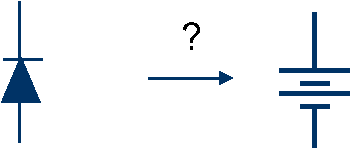
\includegraphics[width=.35\columnwidth]{slide25} & \hspace{.5cm} &
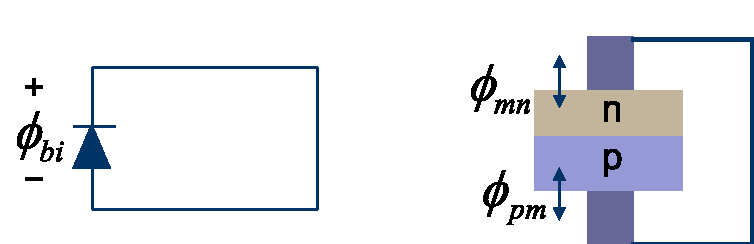
\includegraphics[width=.5\columnwidth]{slide26}\\
(a) &  & (b)\\
\end{tabular}
\caption{(a) One may question if a $PN$-junction is like a battery that can supply power to a circuit.  (b) If we short circuit a $PN$-junction, no current flows because the contact potentials between the metal and the semiconductor perfectly balances the built-in potential. }
\label{fig:slide25_26}
\end{figure}
%%%%%%%%%%%%%%%%%%%%%%%%%%%%%%%%%%%%%%%%%%%%
%             SUBSECTION 5.4.7             %
%%%%%%%%%%%%%%%%%%%%%%%%%%%%%%%%%%%%%%%%%%%%
\subsection{Contact Potential}
%%%%%%%%%%%%%%%%%%%%%%%%%%%%%%%%%%%%%%%%%%%%
%              SUB-SUBSECTION              %
%%%%%%%%%%%%%%%%%%%%%%%%%%%%%%%%%%%%%%%%%%%%
\subsubsection{Have we invented a battery?}
Can we harness the $PN$-junction and turn it into a battery \big(see \emph{Fig.~\ref{fig:slide25_26}(a)}\big).  It seems that we have a perpetual motion machine because our solution to the problem so far does not require any input energy (light for example), and yet we have a potential barrier that maybe can be harnessed to do work.  Why is it that the built-in potential is not a battery?

Unfortunately this cannot be the case.  When we attach a wire to the $PN$-junction, we actually are replaying the same physics that we just described.  For example, a metal is kind of like an $N$-type region, but with very heavy doping.  So it will form a built-in potential, called the \textbf{contact potential}\index{PN-junction!contact potential}, between the $P$-type and $N$-type regions.  Let's call the contact potential with the $N$-type region as $\varphi_{mn}$ and the contact potential with the $P$-type region as $\varphi_{mp}$.  

If we short circuit the $PN$-junction \big(\emph{Fig.~\ref{fig:slide25_26}(b)}\big), then going around the loop we have a KVL loop:
    \begin{equation}
        \varphi_{bi} + \varphi_{mn} + \varphi_{pm} = 0
    \end{equation}
We can re-write this as:
    \begin{equation}
        \varphi_{bi} =  \varphi_{mn} - \varphi_{pm} 
    \end{equation}
This shows that the net built-in potential between the $NP$-region is the same, whether we use the metal potential as the reference or intrinsic silicon as the reference as we did earlier.  

Stated another way, a certain amount of energy is required to take an electron from the semiconductor and put it in the metal, and then back into the semiconductor.  This energy must exactly balance out the built-in potential barrier between the $N$ and $P$ regions, because we are simply providing another pathway for carriers to diffuse across the barrier.  If this pathway did not present a potential barrier,  then we would not be in thermal equilibrium and there would be a net current flow across the junctions from the wire.
%%%%%%%%%%%%%%%%%%%%%%%%%%%%%%%%%%%%%%%%%%%%
%              SUB-SUBSECTION              %
%%%%%%%%%%%%%%%%%%%%%%%%%%%%%%%%%%%%%%%%%%%%
\subsubsection{Contact Potential Between Materials}
In summary, the contact between a $PN$-junction creates a potential difference.    Likewise, the contact between two dissimilar metals creates a potential difference.\footnote{Proportional to the difference between the \textbf{work functions}\index{Work function}.}   When a metal semiconductor junction is formed, a contact potential forms as well.  In fact, forming a good "ohmic" contact\index{Ohmic contact} between a semiconductor and a metal requires special engineering that we usually ignore in an elementary coverage of $PN$-junctions.   
\newpage
%%%%%%%%%%%%%%%%%%%%%%%%%%%%%%%%%%%%%%%%%%%%
%                 FIGURE                   %
%%%%%%%%%%%%%%%%%%%%%%%%%%%%%%%%%%%%%%%%%%%%
\begin{figure}[t]
\centering
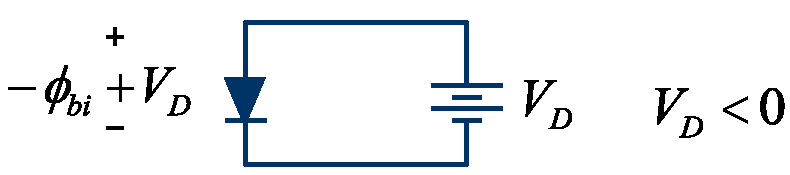
\includegraphics[width=.65\columnwidth]{slide28}
\caption{A voltage $V_D$ is applied across the $PN$-junction.  When the voltage $V_D < 0$V, we say the junction is reverse biased.}
\label{fig:slide28}
\end{figure}
%%%%%%%%%%%%%%%%%%%%%%%%%%%%%%%%%%%%%%%%%%%%
%             SUBSECTION 5.4.8             %
%%%%%%%%%%%%%%%%%%%%%%%%%%%%%%%%%%%%%%%%%%%%
\subsection{\emph{PN}-Junction Capacitor}
Under thermal equilibrium, the $PN$-junction does not draw any current.   But notice that a $PN$-junction stores charge in the space charge region (transition region).   Since the device is storing charge, it is acting like a capacitor.  Positive charge is stored in the $N$-region, and negative charge is stored in the $P$-region:
    \begin{equation} 
        -Q_p = q\,N_A\,x_{p_0} = q\,N_D\,x_{n_0} = (+)Q_n
    \end{equation}
%%%%%%%%%%%%%%%%%%%%%%%%%%%%%%%%%%%%%%%%%%%%%%%%%%%%%%%%%%%%%%%%%%%%%%%%%%%%%%%%%%%%%%%%
%%%%%%%%%%%%%%%%%%%%%%%%%%%%%%%%%%%%%%%%%%%%%%%%%%%%%%%%%%%%%%%%%%%%%%%%%%%%%%%%%%%%%%%%
%                                   SECTION 5.5                                        %
%%%%%%%%%%%%%%%%%%%%%%%%%%%%%%%%%%%%%%%%%%%%%%%%%%%%%%%%%%%%%%%%%%%%%%%%%%%%%%%%%%%%%%%%
%%%%%%%%%%%%%%%%%%%%%%%%%%%%%%%%%%%%%%%%%%%%%%%%%%%%%%%%%%%%%%%%%%%%%%%%%%%%%%%%%%%%%%%%
\section{Reverse Biased PN Junction}
What happens if we \textbf{“reverse-bias”}\index{PN-junction!reverse-bias} the $PN$-junction, as shown in \emph{Fig.~\ref{fig:slide28}}?  Since no current is flowing, the entire reverse biased potential is dropped across the transition region.\footnote{As we will see in the next chapter, a very small amount of current will flow under reverse-bias conditions.}  To accommodate the extra potential, the charge in these regions must increase.  If no current is flowing, the only way for the charge to increase (decrease) is to grow (shrink) the depletion regions.
%%%%%%%%%%%%%%%%%%%%%%%%%%%%%%%%%%%%%%%%%%%%
%             SUBSECTION 5.5.1             %
%%%%%%%%%%%%%%%%%%%%%%%%%%%%%%%%%%%%%%%%%%%%
\subsection{Voltage Dependence of Depletion Width}
We can redo the math, but in the end we realize that the equations are the same except that we replace the built-in potential with the effective reverse bias ($V_D < 0$V).  The depletion regions \emph{grow} (this is how we check our sign convention):
    \begin{equation} 
        x_n(V_D) = \sqrt{ \frac{2\,\varepsilon_s\,(\varphi_{bi} - V_D)}{q\,N_D} \left( \frac{N_A}{N_A + N_D} \right) } = 
        x_{n_0}\,\sqrt{ 1 - \frac{V_D}{\varphi_{bi}} } 
    \end{equation}
and:
    \begin{equation} 
        x_p(V_D) = \sqrt{ \frac{2\,\varepsilon_s\,(\varphi_{bi} - V_D)}{q\,N_A} \left( \frac{N_D}{N_A + N_D} \right) } = 
        x_{p_0}\,\sqrt{ 1 - \frac{V_D}{\varphi_{bi}} } 
    \end{equation}
So the total depletion width is given by:
    \begin{equation}
        X_{dep}(V_D) = x_p(V_D) + x_n(V_D) = 
        \sqrt{ \frac{2\,\varepsilon_s(\varphi_{bi} - V_D)}{q} \left( \frac{1}{N_A} + \frac{1}{N_D} \right) } 
    \end{equation}
We can simplify this equation and write the depletion region width in terms of the zero bias case, $X_{{dep}_0}$, and the applied reverse bias voltage:
    \begin{equation} 
        X_{dep}(V_D) = X_{{dep}_0}\,\sqrt{ 1 - \frac{V_D}{\phi_{bi}}} 
    \end{equation}
%%%%%%%%%%%%%%%%%%%%%%%%%%%%%%%%%%%%%%%%%%%%
%             SUBSECTION 5.5.2             %
%%%%%%%%%%%%%%%%%%%%%%%%%%%%%%%%%%%%%%%%%%%%
\subsection{Charge Versus Bias}
As we increase the reverse bias, the depletion region grows to accommodate more charge ($V_D < 0\,V$):
    \begin{equation} 
        Q_j(V_D) =  -q\,N_A\,x_p(V_D) = -q\,N_A\,x_{p_0}\sqrt{ 1 - \frac{V_D}{\varphi_{bi}} }
    \end{equation}
More charge is stored as we increase the applied voltage, but charge is \textit{not} a linear function of voltage.  This is a non-linear capacitor that we alluded to in the previous chapter.  We can define an incremental \textbf{"small signal" capacitance}\index{Small-signal!capacitance} for small signals by breaking up the charge into two terms:
    \begin{equation} 
        Q_j(V_D + v_D) = Q_j(V_D) + q(v_D) 
    \end{equation}
In the above equation the voltage $v_D$ is a small incremental voltage, $|v_D/V_D| \ll 1$.
%%%%%%%%%%%%%%%%%%%%%%%%%%%%%%%%%%%%%%%%%%%%
%             SUBSECTION 5.5.3             %
%%%%%%%%%%%%%%%%%%%%%%%%%%%%%%%%%%%%%%%%%%%%
\subsection{Derivation of Small Signal Capacitance}
We perform a Taylor Series expansion\index{Taylor expansion} about a fixed operating point $V_D$:
    \begin{equation} 
        Q_j(V_D + v_D) = Q_j(V_D) + \frac{{dQ}_D}{dV} \bigg\rvert_{V_D}{v_D} + \cdots
    \end{equation}
The linear term looks like a regular linear capacitor.  This term is the small-signal capacitance:
    \begin{equation} 
        C_j = C_j(V_D) = \frac{{dQ}_j}{dV} \bigg\rvert_{V = V_D} = 
        \frac{d}{dV} \Bigg( q\,N_A\,x_{p_0} \sqrt{ 1 - \frac{V}{\varphi_{bi}} }\;\Bigg) \Bigg\rvert_{V = V_R}
    \end{equation}
    \begin{equation}
        C_j = \frac{q\,N_A\,x_{p_0}}{2\,\varphi_{bi}\,\sqrt{1 - \frac{V_D}{\varphi_{bi}} }} = 
        \frac{C_{j0}}{\sqrt{ 1 - \frac{V_D}{\varphi_{bi}} }} 
    \end{equation}
The capacitance at zero bias can be written as:
    \begin{equation} 
        C_{j0} = \frac{q\,N_A\,x_{p_0}}{2\,\varphi_{bi}} = 
        \frac{q\,N_A}{2\varphi_{bi}}\sqrt{ \left( \frac{2\,\varepsilon_s\,\varphi_{bi}}{q\,N_A} \right)
            \left( \frac{N_D}{N_A + N_D} \right)} =
            \sqrt{ \frac{q\,\varepsilon_s}{2\,\varphi_{bi}}\,\frac{N_A\,N_D}{N_A + N_D} }
        \label{eq:cj0}
    \end{equation}
%%%%%%%%%%%%%%%%%%%%%%%%%%%%%%%%%%%%%%%%%%%%
%             SUBSECTION 5.5.4             %
%%%%%%%%%%%%%%%%%%%%%%%%%%%%%%%%%%%%%%%%%%%%
\subsection{Physical Interpretation of Depletion Cap}
Notice that the expression on the right-hand-side of \emph{Eq.~\ref{eq:cj0}} is almost just the (inverse) of the depletion width in thermal equilibrium.  A simple manipulation shows that:
    \begin{equation} 
        C_{j0} = \varepsilon_s\,\sqrt{ \frac{q}{2\,\varepsilon_s\,\varphi_{bi}} \left( \frac{1}{N_A} + \frac{1}{N_D} \right) }^{-1} =
        \frac{\varepsilon_s}{X_{{dep}_0}}
    \end{equation}
This looks like a parallel plate capacitor, with capacitance per unit area $C = \epsilon/d$, where $d$ is the distance between the plates. Is that a coincidence?  No, it is actually related to the fact that the incremental charge comes from the edges of the depletion region (as it grows into the $N$-type and $P$-type regions).  So the new incremental charges are separated by a distance of $X_{{dep}_0}$, as if there were plates of metal at the edges of the depletion region.  The depletion region itself looks like a dielectric of permittivity of $\varepsilon_s$ (for silicon $\varepsilon_s = 11.7 \varepsilon_0$.  With this observation, we can state that the small-signal incremental capacitance for an applied reverse-bias voltage $V_D$ is given by:
    \begin{equation} 
        C_j^(V_D) = \frac{\varepsilon_s}{X_{dep}(V_D)} 
    \end{equation}
\newpage
%%%%%%%%%%%%%%%%%%%%%%%%%%%%%%%%%%%%%%%%%%%%
%             SUBSECTION 5.5.5             %
%%%%%%%%%%%%%%%%%%%%%%%%%%%%%%%%%%%%%%%%%%%%
\subsection{A Variable Capacitor (Varactor)}
%%%%%%%%%%%%%%%%%%%%%%%%%%%%%%%%%%%%%%%%%%%%
A good application of the reverse-biased $PN$-junction is a \textbf{"varactor"}\index{Varactor}, or a variable capacitor.  This is used in almost every radio to tune an oscillator to a frequency for transmission and reception of radio waves (for example in a modulator and demodulator).  This is true from a humble AM or FM radio to the most sophisticated modem used for wireless data communication.  As shown in \emph{Fig.~\ref{fig:slide33}}, the capacitance varies in a non-linear way with applied bias $V_c$.  For modern frequency synthesizers, this is not an issue because the applied voltage on the $PN$-junction is derived from a feedback loop that ensures the oscillator is generating zero crossings at a rate consistent with the desired output frequency.\footnote{This is done by comparing edge arrival times to a precision lower frequency reference signal derived from either the received signal  transitions or an accurate clock reference derived from a crystal oscillator.}
%%%%%%%%%%%%%%%%%%%%%%%%%%%%%%%%%%%%%%%%%%%%
%                 FIGURE                   %
%%%%%%%%%%%%%%%%%%%%%%%%%%%%%%%%%%%%%%%%%%%%
\begin{figure}[H]
\centering
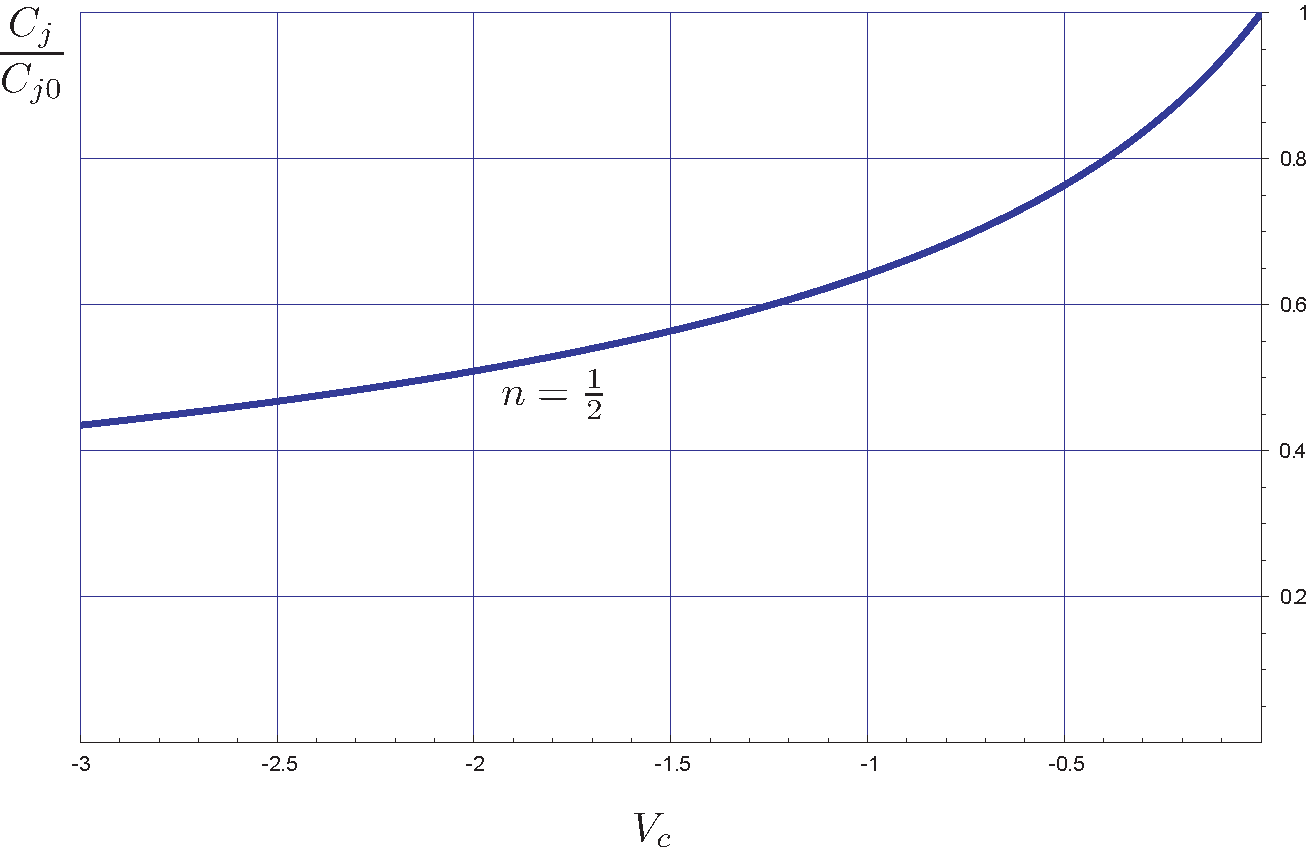
\includegraphics[width=.85\columnwidth]{slide33}\\
(a)\\
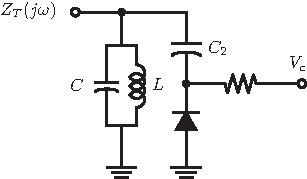
\includegraphics[width=.55\columnwidth]{lctank_varac}\\
(b)\\
\caption{(a) The capacitance as a function of reverse bias voltage.  This result holds for an abrupt junction. (b)  This structure is often used to tune the center frequency of an $LC$ tank to build a voltage controlled oscillator.  The control voltage $V_c$ is the reverse bias DC voltage, and $C_2$ is needed to DC isolate the varactor from the tank.}
\label{fig:slide33}
\end{figure}
%%%%%%%%%%%%%%%%%%%%%%%%%%%%%%%%%%%%%%%%%%%%
% \newpage
% %%%%%%%%%%%%%%%%%%%%%%%%%%%%%%%%%%%%%%%%%%%%%%%%%%%%%%%%%%%%%%%%%%%%%%%%%%%%%%%%%%%%%%%%
% %%%%%%%%%%%%%%%%%%%%%%%%%%%%%%%%%%%%%%%%%%%%%%%%%%%%%%%%%%%%%%%%%%%%%%%%%%%%%%%%%%%%%%%%
% %                                   SECTION 5.6                                        %
% %%%%%%%%%%%%%%%%%%%%%%%%%%%%%%%%%%%%%%%%%%%%%%%%%%%%%%%%%%%%%%%%%%%%%%%%%%%%%%%%%%%%%%%%
% %%%%%%%%%%%%%%%%%%%%%%%%%%%%%%%%%%%%%%%%%%%%%%%%%%%%%%%%%%%%%%%%%%%%%%%%%%%%%%%%%%%%%%%%
% \section{Chapter Summary}
% In this chapter we ...
